\documentclass{../ucll-slides}
\usepackage{../pvm}
\usepackage{siunitx}
\usepackage{ifthen}

\usetikzlibrary{positioning}

\makeatletter
\def\light@caption@on{on}
\def\light@caption@off{off}
\def\light@caption@neutral{}
\makeatother

\tikzset{
  light/.pic={\draw node[circle,#1,minimum size=7mm,font=\tiny] {\csname light@caption@#1\endcsname};},
  light/.style={draw},
  on/.style={light,fill=yellow},
  off/.style={light,fill=gray!50},
  neutral/.style={light}
}

\title{Data Compression: Huffman}
\author{Fr\'ed\'eric Vogels}

\begin{document}

\begin{frame}
  \titlepage
\end{frame}

\begin{frame}
  \frametitle{Disclaimer}
  \begin{center}
    \Large
    Most examples assume we deal with text,
    but the principles apply to bytes in general
  \end{center}
\end{frame}

{
  \newcommand{\freq}[2]{#1 & \SI{#2}{} \\}
  \begin{frame}
    \frametitle{Letter Frequency in ``A Game of Thrones''}

    \begin{columns}
      \column{4cm}
      \begin{center}
        \begin{tabular}{cc}
          \textbf{Letter} & \textbf{Frequency} \\
          \toprule
          \freq{E}{154148}
          \freq{T}{101753}
          \freq{A}{98313}
          \freq{O}{92254}
          \freq{H}{86942}
          \freq{N}{81018}
          \freq{S}{80389}
          \freq{R}{78068}
          \freq{I}{71945}
          \freq{D}{65816}
          \freq{L}{53882}
          \freq{W}{32485}
          \freq{U}{29804}
        \end{tabular}
      \end{center}

      \column{4cm}
      \begin{center}
        \begin{tabular}{cc}
          \textbf{Letter} & \textbf{Frequency} \\
          \toprule
          \freq{M}{29129}
          \freq{G}{27193}
          \freq{Y}{25888}
          \freq{F}{25074}
          \freq{C}{22459}
          \freq{B}{20154}
          \freq{P}{14831}
          \freq{K}{14469}
          \freq{V}{9068}
          \freq{J}{2513}
          \freq{Q}{1050}
          \freq{Z}{599}
          \freq{X}{591}
        \end{tabular}
      \end{center}
    \end{columns}
  \end{frame}
}

\begin{frame}
  \frametitle{Bits vs Letter Frequency}
  \begin{itemize}
    \item Each letter is represented by a unique 8 bit code (ASCII)
    \item The letter E is used 261$\times$ more often than X
    \item It would make more sense to use less bits for E than for~X
  \end{itemize}
\end{frame}

\begin{frame}
  \frametitle{Using Less Bits}
  \begin{itemize}
    \item Say we use 4 bits for E: \texttt{0101}
    \item EE corresponds to \texttt{01010101}
    \item Problem: {\tt U} is also represented by \texttt{01010101}
    \item Decompressor can't know whether you mean EE of U
    \item It is impossible to simply assign a shorter code to E without introducing ambiguities
    \item In order to encode E with less bits, we need to change more than just E's code
  \end{itemize}
\end{frame}

\begin{frame}
  \frametitle{How To Build An Unambiguous Encoding}
  \begin{itemize}
    \item Visualising helps
    \item First, we represent our codes by a tree
    \item Next, we find out what operations we can apply on a tree
  \end{itemize}
\end{frame}

% \input{8-bit-tree.tex}

\begin{frame}
  \frametitle{Oops}
  \begin{itemize}
    \item That was a bit unwieldy
    \item Let's work with 4 bits instead of 8 bits
  \end{itemize}
\end{frame}

\begin{frame}
  \frametitle{How To Build An Unambiguous Encoding}
  \begin{center}
    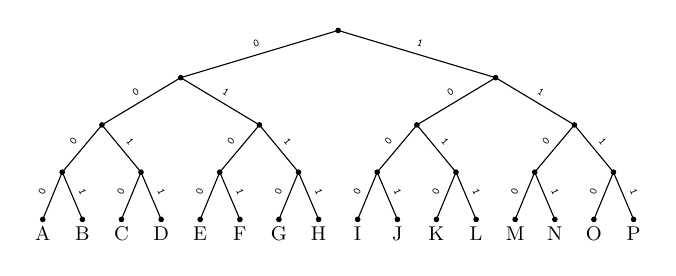
\begin{tikzpicture}[scale=.8,transform shape]
      \draw[fill] (0.0,0.0) circle[radius=1pt] node[below,font=\small] {A};
      \draw[fill] (0.63,0.0) circle[radius=1pt] node[below,font=\small] {B};
      \draw[fill] (1.25,0.0) circle[radius=1pt] node[below,font=\small] {C};
      \draw[fill] (1.88,0.0) circle[radius=1pt] node[below,font=\small] {D};
      \draw[fill] (2.5,0.0) circle[radius=1pt] node[below,font=\small] {E};
      \draw[fill] (3.13,0.0) circle[radius=1pt] node[below,font=\small] {F};
      \draw[fill] (3.75,0.0) circle[radius=1pt] node[below,font=\small] {G};
      \draw[fill] (4.38,0.0) circle[radius=1pt] node[below,font=\small] {H};
      \draw[fill] (5.0,0.0) circle[radius=1pt] node[below,font=\small] {I};
      \draw[fill] (5.63,0.0) circle[radius=1pt] node[below,font=\small] {J};
      \draw[fill] (6.25,0.0) circle[radius=1pt] node[below,font=\small] {K};
      \draw[fill] (6.88,0.0) circle[radius=1pt] node[below,font=\small] {L};
      \draw[fill] (7.5,0.0) circle[radius=1pt] node[below,font=\small] {M};
      \draw[fill] (8.13,0.0) circle[radius=1pt] node[below,font=\small] {N};
      \draw[fill] (8.75,0.0) circle[radius=1pt] node[below,font=\small] {O};
      \draw[fill] (9.38,0.0) circle[radius=1pt] node[below,font=\small] {P};
      \draw (0.0,0.0) -- (0.31,0.75) node[midway,above,sloped,font=\tiny] {\tt 0};
      \draw (0.63,0.0) -- (0.31,0.75) node[midway,above,sloped,font=\tiny] {\tt 1};
      \draw (1.25,0.0) -- (1.56,0.75) node[midway,above,sloped,font=\tiny] {\tt 0};
      \draw (1.88,0.0) -- (1.56,0.75) node[midway,above,sloped,font=\tiny] {\tt 1};
      \draw (2.5,0.0) -- (2.81,0.75) node[midway,above,sloped,font=\tiny] {\tt 0};
      \draw (3.13,0.0) -- (2.81,0.75) node[midway,above,sloped,font=\tiny] {\tt 1};
      \draw (3.75,0.0) -- (4.06,0.75) node[midway,above,sloped,font=\tiny] {\tt 0};
      \draw (4.38,0.0) -- (4.06,0.75) node[midway,above,sloped,font=\tiny] {\tt 1};
      \draw (5.0,0.0) -- (5.31,0.75) node[midway,above,sloped,font=\tiny] {\tt 0};
      \draw (5.63,0.0) -- (5.31,0.75) node[midway,above,sloped,font=\tiny] {\tt 1};
      \draw (6.25,0.0) -- (6.56,0.75) node[midway,above,sloped,font=\tiny] {\tt 0};
      \draw (6.88,0.0) -- (6.56,0.75) node[midway,above,sloped,font=\tiny] {\tt 1};
      \draw (7.5,0.0) -- (7.81,0.75) node[midway,above,sloped,font=\tiny] {\tt 0};
      \draw (8.13,0.0) -- (7.81,0.75) node[midway,above,sloped,font=\tiny] {\tt 1};
      \draw (8.75,0.0) -- (9.06,0.75) node[midway,above,sloped,font=\tiny] {\tt 0};
      \draw (9.38,0.0) -- (9.06,0.75) node[midway,above,sloped,font=\tiny] {\tt 1};
      \draw[fill] (0.31,0.75) circle[radius=1pt];
      \draw[fill] (1.56,0.75) circle[radius=1pt];
      \draw[fill] (2.81,0.75) circle[radius=1pt];
      \draw[fill] (4.06,0.75) circle[radius=1pt];
      \draw[fill] (5.31,0.75) circle[radius=1pt];
      \draw[fill] (6.56,0.75) circle[radius=1pt];
      \draw[fill] (7.81,0.75) circle[radius=1pt];
      \draw[fill] (9.06,0.75) circle[radius=1pt];
      \draw (0.31,0.75) -- (0.94,1.5) node[midway,above,sloped,font=\tiny] {\tt 0};
      \draw (1.56,0.75) -- (0.94,1.5) node[midway,above,sloped,font=\tiny] {\tt 1};
      \draw (2.81,0.75) -- (3.44,1.5) node[midway,above,sloped,font=\tiny] {\tt 0};
      \draw (4.06,0.75) -- (3.44,1.5) node[midway,above,sloped,font=\tiny] {\tt 1};
      \draw (5.31,0.75) -- (5.94,1.5) node[midway,above,sloped,font=\tiny] {\tt 0};
      \draw (6.56,0.75) -- (5.94,1.5) node[midway,above,sloped,font=\tiny] {\tt 1};
      \draw (7.81,0.75) -- (8.44,1.5) node[midway,above,sloped,font=\tiny] {\tt 0};
      \draw (9.06,0.75) -- (8.44,1.5) node[midway,above,sloped,font=\tiny] {\tt 1};
      \draw[fill] (0.94,1.5) circle[radius=1pt];
      \draw[fill] (3.44,1.5) circle[radius=1pt];
      \draw[fill] (5.94,1.5) circle[radius=1pt];
      \draw[fill] (8.44,1.5) circle[radius=1pt];
      \draw (0.94,1.5) -- (2.19,2.25) node[midway,above,sloped,font=\tiny] {\tt 0};
      \draw (3.44,1.5) -- (2.19,2.25) node[midway,above,sloped,font=\tiny] {\tt 1};
      \draw (5.94,1.5) -- (7.19,2.25) node[midway,above,sloped,font=\tiny] {\tt 0};
      \draw (8.44,1.5) -- (7.19,2.25) node[midway,above,sloped,font=\tiny] {\tt 1};
      \draw[fill] (2.19,2.25) circle[radius=1pt];
      \draw[fill] (7.19,2.25) circle[radius=1pt];
      \draw (2.19,2.25) -- (4.69,3.0) node[midway,above,sloped,font=\tiny] {\tt 0};
      \draw (7.19,2.25) -- (4.69,3.0) node[midway,above,sloped,font=\tiny] {\tt 1};
      \draw[fill] (4.69,3.0) circle[radius=1pt];
    \end{tikzpicture}
  \end{center}
  \begin{columns}
    \small
    \column{3cm}
    \begin{center}
      \begin{tabular}{cc}
        \textbf{Letter} & \textbf{Code} \\
        \toprule
        A & \tt 0000 \\
        B & \tt 0001 \\
        C & \tt 0010 \\
        D & \tt 0011 \\
      \end{tabular}
    \end{center}

    \column{3cm}
    \begin{center}
      \begin{tabular}{cc}
        \textbf{Letter} & \textbf{Code} \\
        \toprule
        E & \tt 0100 \\
        F & \tt 0101 \\
        G & \tt 0110 \\
        H & \tt 0111 \\
      \end{tabular}
    \end{center}

    \column{3cm}
    \begin{center}
      \begin{tabular}{cc}
        \textbf{Letter} & \textbf{Code} \\
        \toprule
        I & \tt 1000 \\
        J & \tt 1001 \\
        K & \tt 1010 \\
        L & \tt 1011 \\
      \end{tabular}
    \end{center}

    \column{3cm}
    \begin{center}
      \begin{tabular}{cc}
        \textbf{Letter} & \textbf{Code} \\
        \toprule
        M & \tt 1100 \\
        N & \tt 1101 \\
        O & \tt 1110 \\
        P & \tt 1111 \\
      \end{tabular}
    \end{center}
  \end{columns}
\end{frame}

\begin{frame}
  \frametitle{Modifying the Tree}
  \begin{itemize}
    \item How can we safely modify this tree?
          \vskip4mm
    \item The actual codes do not matter
          \begin{itemize}
            \item Whether A is 0000 or 1111 is not important
          \end{itemize}
          \vskip4mm
    \item What matters to us is
          \begin{itemize}
            \item the \emph{length} of each code
            \item the \emph{unambiguity} of each code
          \end{itemize}
  \end{itemize}
\end{frame}

\begin{frame}
  \frametitle{Swapping Nodes}
  \begin{center}
    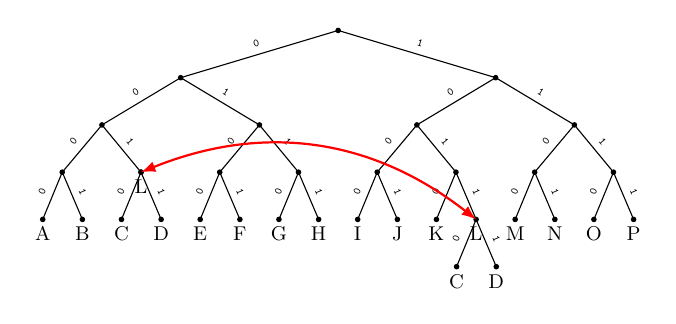
\begin{tikzpicture}[scale=.8,transform shape]
      \draw[fill] (0.0,0.0) circle[radius=1pt] node[below,font=\small] {A};
      \draw[fill] (0.63,0.0) circle[radius=1pt] node[below,font=\small] {B};
      \draw[fill] (2.5,0.0) circle[radius=1pt] node[below,font=\small] {E};
      \draw[fill] (3.13,0.0) circle[radius=1pt] node[below,font=\small] {F};
      \draw[fill] (3.75,0.0) circle[radius=1pt] node[below,font=\small] {G};
      \draw[fill] (4.38,0.0) circle[radius=1pt] node[below,font=\small] {H};
      \draw[fill] (5.0,0.0) circle[radius=1pt] node[below,font=\small] {I};
      \draw[fill] (5.63,0.0) circle[radius=1pt] node[below,font=\small] {J};
      \draw[fill] (6.25,0.0) circle[radius=1pt] node[below,font=\small] {K};
      \draw[fill] (7.5,0.0) circle[radius=1pt] node[below,font=\small] {M};
      \draw[fill] (8.13,0.0) circle[radius=1pt] node[below,font=\small] {N};
      \draw[fill] (8.75,0.0) circle[radius=1pt] node[below,font=\small] {O};
      \draw[fill] (9.38,0.0) circle[radius=1pt] node[below,font=\small] {P};
      \draw (0.0,0.0) -- (0.31,0.75) node[midway,above,sloped,font=\tiny] {\tt 0};
      \draw (0.63,0.0) -- (0.31,0.75) node[midway,above,sloped,font=\tiny] {\tt 1};
      \draw (2.5,0.0) -- (2.81,0.75) node[midway,above,sloped,font=\tiny] {\tt 0};
      \draw (3.13,0.0) -- (2.81,0.75) node[midway,above,sloped,font=\tiny] {\tt 1};
      \draw (3.75,0.0) -- (4.06,0.75) node[midway,above,sloped,font=\tiny] {\tt 0};
      \draw (4.38,0.0) -- (4.06,0.75) node[midway,above,sloped,font=\tiny] {\tt 1};
      \draw (5.0,0.0) -- (5.31,0.75) node[midway,above,sloped,font=\tiny] {\tt 0};
      \draw (5.63,0.0) -- (5.31,0.75) node[midway,above,sloped,font=\tiny] {\tt 1};
      \draw (6.25,0.0) -- (6.56,0.75) node[midway,above,sloped,font=\tiny] {\tt 0};
      \draw (6.88,0.0) -- (6.56,0.75) node[midway,above,sloped,font=\tiny] {\tt 1};
      \draw (7.5,0.0) -- (7.81,0.75) node[midway,above,sloped,font=\tiny] {\tt 0};
      \draw (8.13,0.0) -- (7.81,0.75) node[midway,above,sloped,font=\tiny] {\tt 1};
      \draw (8.75,0.0) -- (9.06,0.75) node[midway,above,sloped,font=\tiny] {\tt 0};
      \draw (9.38,0.0) -- (9.06,0.75) node[midway,above,sloped,font=\tiny] {\tt 1};
      \draw[fill] (0.31,0.75) circle[radius=1pt];
      \draw[fill] (1.56,0.75) circle[radius=1pt];
      \draw[fill] (2.81,0.75) circle[radius=1pt];
      \draw[fill] (4.06,0.75) circle[radius=1pt];
      \draw[fill] (5.31,0.75) circle[radius=1pt];
      \draw[fill] (6.56,0.75) circle[radius=1pt];
      \draw[fill] (7.81,0.75) circle[radius=1pt];
      \draw[fill] (9.06,0.75) circle[radius=1pt];
      \draw (0.31,0.75) -- (0.94,1.5) node[midway,above,sloped,font=\tiny] {\tt 0};
      \draw (1.56,0.75) -- (0.94,1.5) node[midway,above,sloped,font=\tiny] {\tt 1};
      \draw (2.81,0.75) -- (3.44,1.5) node[midway,above,sloped,font=\tiny] {\tt 0};
      \draw (4.06,0.75) -- (3.44,1.5) node[midway,above,sloped,font=\tiny] {\tt 1};
      \draw (5.31,0.75) -- (5.94,1.5) node[midway,above,sloped,font=\tiny] {\tt 0};
      \draw (6.56,0.75) -- (5.94,1.5) node[midway,above,sloped,font=\tiny] {\tt 1};
      \draw (7.81,0.75) -- (8.44,1.5) node[midway,above,sloped,font=\tiny] {\tt 0};
      \draw (9.06,0.75) -- (8.44,1.5) node[midway,above,sloped,font=\tiny] {\tt 1};
      \draw[fill] (0.94,1.5) circle[radius=1pt];
      \draw[fill] (3.44,1.5) circle[radius=1pt];
      \draw[fill] (5.94,1.5) circle[radius=1pt];
      \draw[fill] (8.44,1.5) circle[radius=1pt];
      \draw (0.94,1.5) -- (2.19,2.25) node[midway,above,sloped,font=\tiny] {\tt 0};
      \draw (3.44,1.5) -- (2.19,2.25) node[midway,above,sloped,font=\tiny] {\tt 1};
      \draw (5.94,1.5) -- (7.19,2.25) node[midway,above,sloped,font=\tiny] {\tt 0};
      \draw (8.44,1.5) -- (7.19,2.25) node[midway,above,sloped,font=\tiny] {\tt 1};
      \draw[fill] (2.19,2.25) circle[radius=1pt];
      \draw[fill] (7.19,2.25) circle[radius=1pt];
      \draw (2.19,2.25) -- (4.69,3.0) node[midway,above,sloped,font=\tiny] {\tt 0};
      \draw (7.19,2.25) -- (4.69,3.0) node[midway,above,sloped,font=\tiny] {\tt 1};
      \draw[fill] (4.69,3.0) circle[radius=1pt];

      \visible<1-2>{
        \draw[fill] (1.25,0.0) circle[radius=1pt] node[below,font=\small] {C};
        \draw[fill] (1.88,0.0) circle[radius=1pt] node[below,font=\small] {D};
        \draw (1.25,0.0) -- (1.56,0.75) node[midway,above,sloped,font=\tiny] {\tt 0};
        \draw (1.88,0.0) -- (1.56,0.75) node[midway,above,sloped,font=\tiny] {\tt 1};
        \draw[fill] (6.88,0.0) circle[radius=1pt] node[below,font=\small] {L};
      }

      \visible<3>{
        \begin{scope}[xshift=-1.56cm,yshift=-0.75cm,xshift=6.88cm]
          \draw[fill] (1.25,0.0) circle[radius=1pt] node[below,font=\small] {C};
          \draw[fill] (1.88,0.0) circle[radius=1pt] node[below,font=\small] {D};
          \draw (1.25,0.0) -- (1.56,0.75) node[midway,above,sloped,font=\tiny] {\tt 0};
          \draw (1.88,0.0) -- (1.56,0.75) node[midway,above,sloped,font=\tiny] {\tt 1};
        \end{scope}

        \draw[fill] (1.56,0.75) circle[radius=1pt] node[below,font=\small] {L};
      }

      \visible<2>{
        \draw[latex-latex,red,thick] (1.56,0.75) to [bend left=30] (6.88,0.0);
      }
    \end{tikzpicture}
  \end{center}

  \begin{columns}
    \small
    \column{3cm}
    \begin{center}
      \begin{tabular}{cc}
        \textbf{Letter} & \textbf{Code} \\
        \toprule
        A & \tt 0000 \\
        B & \tt 0001 \\
        C & \tt \alt<1-2>{0010}{\color{red}10110} \\
        D & \tt \alt<1-2>{0011}{\color{red}10111} \\
      \end{tabular}
    \end{center}

    \column{3cm}
    \begin{center}
      \begin{tabular}{cc}
        \textbf{Letter} & \textbf{Code} \\
        \toprule
        E & \tt 0100 \\
        F & \tt 0101 \\
        G & \tt 0110 \\
        H & \tt 0111 \\
      \end{tabular}
    \end{center}

    \column{3cm}
    \begin{center}
      \begin{tabular}{cc}
        \textbf{Letter} & \textbf{Code} \\
        \toprule
        I & \tt 1000 \\
        J & \tt 1001 \\
        K & \tt 1010 \\
        L & \tt \alt<1-2>{1011}{\color{red}001} \\
      \end{tabular}
    \end{center}

    \column{3cm}
    \begin{center}
      \begin{tabular}{cc}
        \textbf{Letter} & \textbf{Code} \\
        \toprule
        M & \tt 1100 \\
        N & \tt 1101 \\
        O & \tt 1110 \\
        P & \tt 1111 \\
      \end{tabular}
    \end{center}
  \end{columns}
\end{frame}

\begin{frame}
  \frametitle{Swapping Nodes}
  \begin{itemize}
    \item We can swap any two nodes in the tree
    \item The resulting code remains unambiguous
    \item The codes have changed
          \begin{itemize}
            \item L's code became 1 bit shorter
            \item C and D's codes became 1 bit longer
            \item Gain 1 bit but lose 2: typical for compression
          \end{itemize}
    \item Goal of swapping:
          \begin{itemize}
            \item Make frequent letters have shorter codes
            \item Sacrifice rarely occurring letters
          \end{itemize}
  \end{itemize}
\end{frame}

\begin{frame}
  \frametitle{Optimal Tree}
  \begin{center} \small
    \begin{tabular}{cc@{\hspace{5mm}}cc@{\hspace{5mm}}cc@{\hspace{5mm}}cc}
      \textbf{Letter} & \textbf{\#} & \textbf{Letter} & \textbf{\#} & \textbf{Letter} & \textbf{\#} & \textbf{Letter} & \textbf{\#} \\
      \toprule
      A & 98 & E & 154 & I & 72 & M & 29 \\
      B & 20 & F & 254 & J & 3 & N & 81 \\
      C & 22 & G & 27 & K & 14 & O & 92 \\
      D & 66 & H & 87 & L & 54 & P & 15 \\
    \end{tabular}
  \end{center}

  \begin{itemize}
    \item E occurs most often
    \item J and P appear least often
    \item We can ``steal'' from J and P and give to E
          \begin{itemize}
            \item E: 3 bits
            \item P, J: 5 bits
          \end{itemize}
  \end{itemize}
\end{frame}

\begin{frame}
  \frametitle{Optimal Tree}
  \begin{overprint}
    \onslide<1>
    \begin{center}
      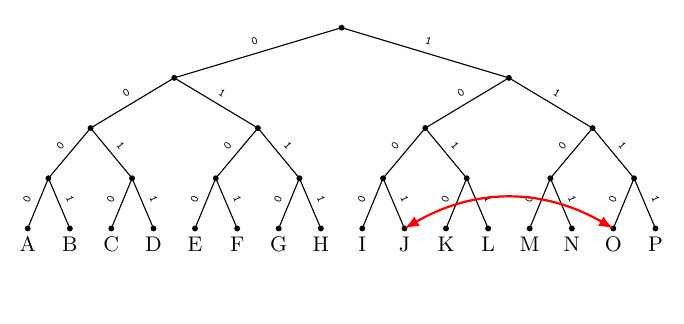
\begin{tikzpicture}[scale=.85,transform shape]
        \path[use as bounding box] (0,-1) rectangle (9.38,3);
        \draw[fill] (0.0,0.0) circle[radius=1pt] node[below,font=\small] {A};
        \draw[fill] (0.63,0.0) circle[radius=1pt] node[below,font=\small] {B};
        \draw[fill] (1.25,0.0) circle[radius=1pt] node[below,font=\small] {C};
        \draw[fill] (1.88,0.0) circle[radius=1pt] node[below,font=\small] {D};
        \draw[fill] (2.5,0.0) circle[radius=1pt] node[below,font=\small] {E};
        \draw[fill] (3.13,0.0) circle[radius=1pt] node[below,font=\small] {F};
        \draw[fill] (3.75,0.0) circle[radius=1pt] node[below,font=\small] {G};
        \draw[fill] (4.38,0.0) circle[radius=1pt] node[below,font=\small] {H};
        \draw[fill] (5.0,0.0) circle[radius=1pt] node[below,font=\small] {I};
        \draw[fill] (5.63,0.0) circle[radius=1pt] node[below,font=\small] {J};
        \draw[fill] (6.25,0.0) circle[radius=1pt] node[below,font=\small] {K};
        \draw[fill] (6.88,0.0) circle[radius=1pt] node[below,font=\small] {L};
        \draw[fill] (7.5,0.0) circle[radius=1pt] node[below,font=\small] {M};
        \draw[fill] (8.13,0.0) circle[radius=1pt] node[below,font=\small] {N};
        \draw[fill] (8.75,0.0) circle[radius=1pt] node[below,font=\small] {O};
        \draw[fill] (9.38,0.0) circle[radius=1pt] node[below,font=\small] {P};
        \draw (0.0,0.0) -- (0.31,0.75) node[midway,above,sloped,font=\tiny] {\tt 0};
        \draw (0.63,0.0) -- (0.31,0.75) node[midway,above,sloped,font=\tiny] {\tt 1};
        \draw (1.25,0.0) -- (1.56,0.75) node[midway,above,sloped,font=\tiny] {\tt 0};
        \draw (1.88,0.0) -- (1.56,0.75) node[midway,above,sloped,font=\tiny] {\tt 1};
        \draw (2.5,0.0) -- (2.81,0.75) node[midway,above,sloped,font=\tiny] {\tt 0};
        \draw (3.13,0.0) -- (2.81,0.75) node[midway,above,sloped,font=\tiny] {\tt 1};
        \draw (3.75,0.0) -- (4.06,0.75) node[midway,above,sloped,font=\tiny] {\tt 0};
        \draw (4.38,0.0) -- (4.06,0.75) node[midway,above,sloped,font=\tiny] {\tt 1};
        \draw (5.0,0.0) -- (5.31,0.75) node[midway,above,sloped,font=\tiny] {\tt 0};
        \draw (5.63,0.0) -- (5.31,0.75) node[midway,above,sloped,font=\tiny] {\tt 1};
        \draw (6.25,0.0) -- (6.56,0.75) node[midway,above,sloped,font=\tiny] {\tt 0};
        \draw (6.88,0.0) -- (6.56,0.75) node[midway,above,sloped,font=\tiny] {\tt 1};
        \draw (7.5,0.0) -- (7.81,0.75) node[midway,above,sloped,font=\tiny] {\tt 0};
        \draw (8.13,0.0) -- (7.81,0.75) node[midway,above,sloped,font=\tiny] {\tt 1};
        \draw (8.75,0.0) -- (9.06,0.75) node[midway,above,sloped,font=\tiny] {\tt 0};
        \draw (9.38,0.0) -- (9.06,0.75) node[midway,above,sloped,font=\tiny] {\tt 1};
        \draw[fill] (0.31,0.75) circle[radius=1pt];
        \draw[fill] (1.56,0.75) circle[radius=1pt];
        \draw[fill] (2.81,0.75) circle[radius=1pt];
        \draw[fill] (4.06,0.75) circle[radius=1pt];
        \draw[fill] (5.31,0.75) circle[radius=1pt];
        \draw[fill] (6.56,0.75) circle[radius=1pt];
        \draw[fill] (7.81,0.75) circle[radius=1pt];
        \draw[fill] (9.06,0.75) circle[radius=1pt];
        \draw (0.31,0.75) -- (0.94,1.5) node[midway,above,sloped,font=\tiny] {\tt 0};
        \draw (1.56,0.75) -- (0.94,1.5) node[midway,above,sloped,font=\tiny] {\tt 1};
        \draw (2.81,0.75) -- (3.44,1.5) node[midway,above,sloped,font=\tiny] {\tt 0};
        \draw (4.06,0.75) -- (3.44,1.5) node[midway,above,sloped,font=\tiny] {\tt 1};
        \draw (5.31,0.75) -- (5.94,1.5) node[midway,above,sloped,font=\tiny] {\tt 0};
        \draw (6.56,0.75) -- (5.94,1.5) node[midway,above,sloped,font=\tiny] {\tt 1};
        \draw (7.81,0.75) -- (8.44,1.5) node[midway,above,sloped,font=\tiny] {\tt 0};
        \draw (9.06,0.75) -- (8.44,1.5) node[midway,above,sloped,font=\tiny] {\tt 1};
        \draw[fill] (0.94,1.5) circle[radius=1pt];
        \draw[fill] (3.44,1.5) circle[radius=1pt];
        \draw[fill] (5.94,1.5) circle[radius=1pt];
        \draw[fill] (8.44,1.5) circle[radius=1pt];
        \draw (0.94,1.5) -- (2.19,2.25) node[midway,above,sloped,font=\tiny] {\tt 0};
        \draw (3.44,1.5) -- (2.19,2.25) node[midway,above,sloped,font=\tiny] {\tt 1};
        \draw (5.94,1.5) -- (7.19,2.25) node[midway,above,sloped,font=\tiny] {\tt 0};
        \draw (8.44,1.5) -- (7.19,2.25) node[midway,above,sloped,font=\tiny] {\tt 1};
        \draw[fill] (2.19,2.25) circle[radius=1pt];
        \draw[fill] (7.19,2.25) circle[radius=1pt];
        \draw (2.19,2.25) -- (4.69,3.0) node[midway,above,sloped,font=\tiny] {\tt 0};
        \draw (7.19,2.25) -- (4.69,3.0) node[midway,above,sloped,font=\tiny] {\tt 1};
        \draw[fill] (4.69,3.0) circle[radius=1pt];

        \draw[thick,red,latex-latex] (5.63,0.0) to[bend left=30] (8.75,0.0);
      \end{tikzpicture}
    \end{center}

    \onslide<2-3>
    \begin{center}
      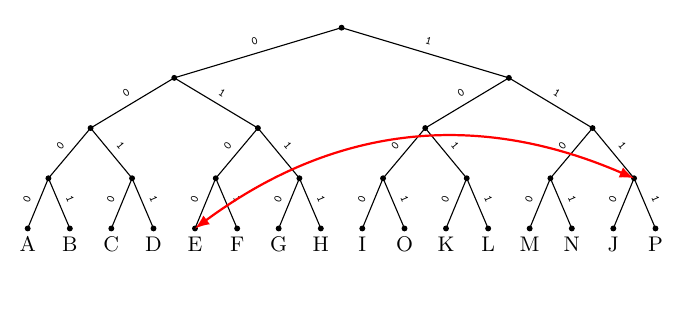
\begin{tikzpicture}[scale=.85,transform shape]
        \path[use as bounding box] (0,-1) rectangle (9.38,3);
        \draw[fill] (0.0,0.0) circle[radius=1pt] node[below,font=\small] {A};
        \draw[fill] (0.63,0.0) circle[radius=1pt] node[below,font=\small] {B};
        \draw[fill] (1.25,0.0) circle[radius=1pt] node[below,font=\small] {C};
        \draw[fill] (1.88,0.0) circle[radius=1pt] node[below,font=\small] {D};
        \draw[fill] (2.5,0.0) circle[radius=1pt] node[below,font=\small] {E};
        \draw[fill] (3.13,0.0) circle[radius=1pt] node[below,font=\small] {F};
        \draw[fill] (3.75,0.0) circle[radius=1pt] node[below,font=\small] {G};
        \draw[fill] (4.38,0.0) circle[radius=1pt] node[below,font=\small] {H};
        \draw[fill] (5.0,0.0) circle[radius=1pt] node[below,font=\small] {I};
        \draw[fill] (5.63,0.0) circle[radius=1pt] node[below,font=\small] {O};
        \draw[fill] (6.25,0.0) circle[radius=1pt] node[below,font=\small] {K};
        \draw[fill] (6.88,0.0) circle[radius=1pt] node[below,font=\small] {L};
        \draw[fill] (7.5,0.0) circle[radius=1pt] node[below,font=\small] {M};
        \draw[fill] (8.13,0.0) circle[radius=1pt] node[below,font=\small] {N};
        \draw[fill] (8.75,0.0) circle[radius=1pt] node[below,font=\small] {J};
        \draw[fill] (9.38,0.0) circle[radius=1pt] node[below,font=\small] {P};
        \draw (0.0,0.0) -- (0.31,0.75) node[midway,above,sloped,font=\tiny] {\tt 0};
        \draw (0.63,0.0) -- (0.31,0.75) node[midway,above,sloped,font=\tiny] {\tt 1};
        \draw (1.25,0.0) -- (1.56,0.75) node[midway,above,sloped,font=\tiny] {\tt 0};
        \draw (1.88,0.0) -- (1.56,0.75) node[midway,above,sloped,font=\tiny] {\tt 1};
        \draw (2.5,0.0) -- (2.81,0.75) node[midway,above,sloped,font=\tiny] {\tt 0};
        \draw (3.13,0.0) -- (2.81,0.75) node[midway,above,sloped,font=\tiny] {\tt 1};
        \draw (3.75,0.0) -- (4.06,0.75) node[midway,above,sloped,font=\tiny] {\tt 0};
        \draw (4.38,0.0) -- (4.06,0.75) node[midway,above,sloped,font=\tiny] {\tt 1};
        \draw (5.0,0.0) -- (5.31,0.75) node[midway,above,sloped,font=\tiny] {\tt 0};
        \draw (5.63,0.0) -- (5.31,0.75) node[midway,above,sloped,font=\tiny] {\tt 1};
        \draw (6.25,0.0) -- (6.56,0.75) node[midway,above,sloped,font=\tiny] {\tt 0};
        \draw (6.88,0.0) -- (6.56,0.75) node[midway,above,sloped,font=\tiny] {\tt 1};
        \draw (7.5,0.0) -- (7.81,0.75) node[midway,above,sloped,font=\tiny] {\tt 0};
        \draw (8.13,0.0) -- (7.81,0.75) node[midway,above,sloped,font=\tiny] {\tt 1};
        \draw (8.75,0.0) -- (9.06,0.75) node[midway,above,sloped,font=\tiny] {\tt 0};
        \draw (9.38,0.0) -- (9.06,0.75) node[midway,above,sloped,font=\tiny] {\tt 1};
        \draw[fill] (0.31,0.75) circle[radius=1pt];
        \draw[fill] (1.56,0.75) circle[radius=1pt];
        \draw[fill] (2.81,0.75) circle[radius=1pt];
        \draw[fill] (4.06,0.75) circle[radius=1pt];
        \draw[fill] (5.31,0.75) circle[radius=1pt];
        \draw[fill] (6.56,0.75) circle[radius=1pt];
        \draw[fill] (7.81,0.75) circle[radius=1pt];
        \draw[fill] (9.06,0.75) circle[radius=1pt];
        \draw (0.31,0.75) -- (0.94,1.5) node[midway,above,sloped,font=\tiny] {\tt 0};
        \draw (1.56,0.75) -- (0.94,1.5) node[midway,above,sloped,font=\tiny] {\tt 1};
        \draw (2.81,0.75) -- (3.44,1.5) node[midway,above,sloped,font=\tiny] {\tt 0};
        \draw (4.06,0.75) -- (3.44,1.5) node[midway,above,sloped,font=\tiny] {\tt 1};
        \draw (5.31,0.75) -- (5.94,1.5) node[midway,above,sloped,font=\tiny] {\tt 0};
        \draw (6.56,0.75) -- (5.94,1.5) node[midway,above,sloped,font=\tiny] {\tt 1};
        \draw (7.81,0.75) -- (8.44,1.5) node[midway,above,sloped,font=\tiny] {\tt 0};
        \draw (9.06,0.75) -- (8.44,1.5) node[midway,above,sloped,font=\tiny] {\tt 1};
        \draw[fill] (0.94,1.5) circle[radius=1pt];
        \draw[fill] (3.44,1.5) circle[radius=1pt];
        \draw[fill] (5.94,1.5) circle[radius=1pt];
        \draw[fill] (8.44,1.5) circle[radius=1pt];
        \draw (0.94,1.5) -- (2.19,2.25) node[midway,above,sloped,font=\tiny] {\tt 0};
        \draw (3.44,1.5) -- (2.19,2.25) node[midway,above,sloped,font=\tiny] {\tt 1};
        \draw (5.94,1.5) -- (7.19,2.25) node[midway,above,sloped,font=\tiny] {\tt 0};
        \draw (8.44,1.5) -- (7.19,2.25) node[midway,above,sloped,font=\tiny] {\tt 1};
        \draw[fill] (2.19,2.25) circle[radius=1pt];
        \draw[fill] (7.19,2.25) circle[radius=1pt];
        \draw (2.19,2.25) -- (4.69,3.0) node[midway,above,sloped,font=\tiny] {\tt 0};
        \draw (7.19,2.25) -- (4.69,3.0) node[midway,above,sloped,font=\tiny] {\tt 1};
        \draw[fill] (4.69,3.0) circle[radius=1pt];

        \only<3>{
          \draw[thick,red,latex-latex] (2.5,0.0) to[bend left=30] (9.06,0.75);
        }
      \end{tikzpicture}
    \end{center}

    \onslide<4->
    \begin{center}
      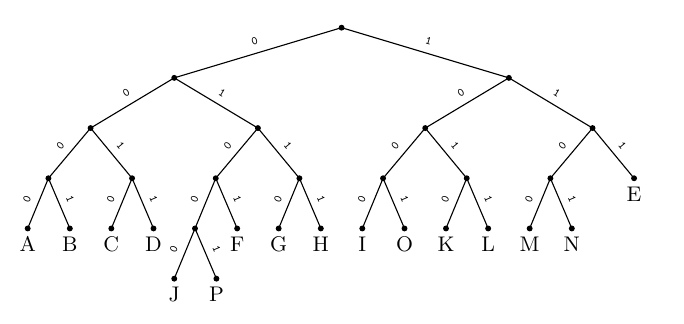
\begin{tikzpicture}[scale=.85,transform shape]
        \path[use as bounding box] (0,-1) rectangle (9.38,3);
        \draw[fill] (0.0,0.0) circle[radius=1pt] node[below,font=\small] {A};
        \draw[fill] (0.63,0.0) circle[radius=1pt] node[below,font=\small] {B};
        \draw[fill] (1.25,0.0) circle[radius=1pt] node[below,font=\small] {C};
        \draw[fill] (1.88,0.0) circle[radius=1pt] node[below,font=\small] {D};
        \draw[fill] (3.13,0.0) circle[radius=1pt] node[below,font=\small] {F};
        \draw[fill] (3.75,0.0) circle[radius=1pt] node[below,font=\small] {G};
        \draw[fill] (4.38,0.0) circle[radius=1pt] node[below,font=\small] {H};
        \draw[fill] (5.0,0.0) circle[radius=1pt] node[below,font=\small] {I};
        \draw[fill] (5.63,0.0) circle[radius=1pt] node[below,font=\small] {O};
        \draw[fill] (6.25,0.0) circle[radius=1pt] node[below,font=\small] {K};
        \draw[fill] (6.88,0.0) circle[radius=1pt] node[below,font=\small] {L};
        \draw[fill] (7.5,0.0) circle[radius=1pt] node[below,font=\small] {M};
        \draw[fill] (8.13,0.0) circle[radius=1pt] node[below,font=\small] {N};
        \draw (0.0,0.0) -- (0.31,0.75) node[midway,above,sloped,font=\tiny] {\tt 0};
        \draw (0.63,0.0) -- (0.31,0.75) node[midway,above,sloped,font=\tiny] {\tt 1};
        \draw (1.25,0.0) -- (1.56,0.75) node[midway,above,sloped,font=\tiny] {\tt 0};
        \draw (1.88,0.0) -- (1.56,0.75) node[midway,above,sloped,font=\tiny] {\tt 1};
        \draw (3.13,0.0) -- (2.81,0.75) node[midway,above,sloped,font=\tiny] {\tt 1};
        \draw (3.75,0.0) -- (4.06,0.75) node[midway,above,sloped,font=\tiny] {\tt 0};
        \draw (4.38,0.0) -- (4.06,0.75) node[midway,above,sloped,font=\tiny] {\tt 1};
        \draw (5.0,0.0) -- (5.31,0.75) node[midway,above,sloped,font=\tiny] {\tt 0};
        \draw (5.63,0.0) -- (5.31,0.75) node[midway,above,sloped,font=\tiny] {\tt 1};
        \draw (6.25,0.0) -- (6.56,0.75) node[midway,above,sloped,font=\tiny] {\tt 0};
        \draw (6.88,0.0) -- (6.56,0.75) node[midway,above,sloped,font=\tiny] {\tt 1};
        \draw (7.5,0.0) -- (7.81,0.75) node[midway,above,sloped,font=\tiny] {\tt 0};
        \draw (8.13,0.0) -- (7.81,0.75) node[midway,above,sloped,font=\tiny] {\tt 1};
        \draw[fill] (0.31,0.75) circle[radius=1pt];
        \draw[fill] (1.56,0.75) circle[radius=1pt];
        \draw[fill] (2.81,0.75) circle[radius=1pt];
        \draw[fill] (4.06,0.75) circle[radius=1pt];
        \draw[fill] (5.31,0.75) circle[radius=1pt];
        \draw[fill] (6.56,0.75) circle[radius=1pt];
        \draw[fill] (7.81,0.75) circle[radius=1pt];
        \draw (0.31,0.75) -- (0.94,1.5) node[midway,above,sloped,font=\tiny] {\tt 0};
        \draw (1.56,0.75) -- (0.94,1.5) node[midway,above,sloped,font=\tiny] {\tt 1};
        \draw (2.81,0.75) -- (3.44,1.5) node[midway,above,sloped,font=\tiny] {\tt 0};
        \draw (4.06,0.75) -- (3.44,1.5) node[midway,above,sloped,font=\tiny] {\tt 1};
        \draw (5.31,0.75) -- (5.94,1.5) node[midway,above,sloped,font=\tiny] {\tt 0};
        \draw (6.56,0.75) -- (5.94,1.5) node[midway,above,sloped,font=\tiny] {\tt 1};
        \draw (7.81,0.75) -- (8.44,1.5) node[midway,above,sloped,font=\tiny] {\tt 0};
        \draw (9.06,0.75) -- (8.44,1.5) node[midway,above,sloped,font=\tiny] {\tt 1};
        \draw[fill] (0.94,1.5) circle[radius=1pt];
        \draw[fill] (3.44,1.5) circle[radius=1pt];
        \draw[fill] (5.94,1.5) circle[radius=1pt];
        \draw[fill] (8.44,1.5) circle[radius=1pt];
        \draw (0.94,1.5) -- (2.19,2.25) node[midway,above,sloped,font=\tiny] {\tt 0};
        \draw (3.44,1.5) -- (2.19,2.25) node[midway,above,sloped,font=\tiny] {\tt 1};
        \draw (5.94,1.5) -- (7.19,2.25) node[midway,above,sloped,font=\tiny] {\tt 0};
        \draw (8.44,1.5) -- (7.19,2.25) node[midway,above,sloped,font=\tiny] {\tt 1};
        \draw[fill] (2.19,2.25) circle[radius=1pt];
        \draw[fill] (7.19,2.25) circle[radius=1pt];
        \draw (2.19,2.25) -- (4.69,3.0) node[midway,above,sloped,font=\tiny] {\tt 0};
        \draw (7.19,2.25) -- (4.69,3.0) node[midway,above,sloped,font=\tiny] {\tt 1};
        \draw[fill] (4.69,3.0) circle[radius=1pt];
        \draw (2.5,0.0) -- (2.81,0.75) node[midway,above,sloped,font=\tiny] {\tt 0};

        \begin{scope}[xshift=-9.06cm,xshift=2.5cm,yshift=-0.75cm]
          \draw[fill] (8.75,0.0) circle[radius=1pt] node[below,font=\small] {J};
          \draw[fill] (9.38,0.0) circle[radius=1pt] node[below,font=\small] {P};
          \draw (8.75,0.0) -- (9.06,0.75) node[midway,above,sloped,font=\tiny] {\tt 0};
          \draw (9.38,0.0) -- (9.06,0.75) node[midway,above,sloped,font=\tiny] {\tt 1};
        \draw[fill] (9.06,0.75) circle[radius=1pt];
        \end{scope}
        \draw[fill] (9.06,0.75) circle[radius=1pt] node[below,font=\small] {E};
      \end{tikzpicture}
    \end{center}
  \end{overprint}
  \begin{itemize}
    \item<1-> We want to make E shorter and P, J longer
    \item<1-> We need to put P and J together somehow
    \item<3-> We can now swap E with P,J
    \item<5> New codes: E=111, J=01000, P=01001
  \end{itemize}
\end{frame}

\begin{frame}
  \frametitle{Optimal Tree}
  \begin{itemize}
    \item Is this new tree optimal?
    \item We could make E two bits long by sacrificing other letters
    \item 
  \end{itemize}
\end{frame}

\end{document}